\section{{\it Hash} perfeito}

\begin{frame}[fragile]{Definição de {\it hash} perfeito}

    \begin{itemize}
        \item Seja um conjunto de chaves $\mathcal{K} = \lbrace K_1, K_2, \ldots, K_N\rbrace$,
            a serem inseridas em uma tabela com tamanho $T$

        \item Uma função $h: \mathcal{K} \to [0, T-1]$ é um \textit{hash} perfeito para 
            $\mathcal{K}$ se para todos os pares de índices $(i, j)$, com $i\neq j$, 
            segue que $h(K_i) \neq h(K_j)$

        \item Veja que a definição de \textit{hash} perfeito depende do conjunto $\mathcal{K}$

        \item Existem $T^N$ funções $h: \mathcal{K}\to [0, T-1]$

        \item Destas, apenas
        \[
            A_{T,N} = \frac{T!}{(T - N)!}
        \]
        são \textit{hashes} perfeitos

        \item Por exemplo, para $T = 100, N = 80$, há $100^{80} = 10^{160}$ funções, dentre as
        quais $A_{100, 80} < 10^{140}$ são \textit{hashes} perfeitos

        \item Logo, uma a cada $10^{20}$ destas funções serão \textit{hashes} perfeitos
    \end{itemize}

\end{frame}

\begin{frame}[fragile]{Construção de um {\it hash} perfeito}

    \begin{itemize}
        \item Embora exista, em valor absoluto, um grande número de \textit{hashes} perfeitos,
            não é tarefa trivial determinar um deles na prática

        \item A maior não tem sequer uma representação óbvia como função

        \item Pode-se construir um \textit{hash} perfeito para o conjunto $\mathcal{K}$
            combinando-se três ideias já apresentadas: encadeamento, \textit{hash} duplo e 
                \textit{hash} universal

        \item O \textit{hash} universal é utilizado para determinar o tamanho das listas
            encadeadas associadas a cada entrada da tabela, segundo o teorema abaixo
    \end{itemize}

    \metroset{block=fill}
    \begin{block}{Teorema}
        Seja $T = N^2$ e $h \in \mathcal{H}_{pT}$. Então a probabilidade de que exista
        colisão entre duas chaves distintas de $\mathcal{K}$ é inferior a $1/2$
    \end{block}
	
\end{frame}

\begin{frame}[fragile]{Construção de um {\it hash} perfeito}

    \begin{itemize}
        \item Se o valor $T = N^2$ for pequeno, é possível encontrar um \textit{hash} perfeito em
            $\mathcal{H}_{pT}$ após algumas tentativas

        \item Porém, para valores grandes de $T$, a ideia é utilizar o encadeamento com
            \textit{hash} duplo

        \item Escolha uma função de \textit{hash} $h$ no conjunto universal $\mathcal{H}_{pN}$
 
        \item Seja $n_j$ o número de chaves $K$ em $\mathcal{K}$ tais que $h(K) = j$, com
            $j = 0, 1, 2, \ldots, N - 1$

        \item A ideia é associar uma nova tabela $t_j$, de 
            tamanho $n_j^2$, para cada célula de uma tabela de tamanho $N$

        \item Os elementos que colidiram na célula $j$ são então mapeados em $T_j$, através de uma
            nova função de \textit{hash} $\hat{h}\in \mathcal{H}_{qn_j^2}$, onde $q$ é um
            primo maior do que $n_j^2$
    \end{itemize}

\end{frame}

\begin{frame}[fragile]{Construção de um {\it hash} perfeito}

    \begin{itemize}
        \item Embora a abordagem descrita leve a crer que o espaço ocupado por todas as 
            tabelas auxiliares $t_i$ seja $O(N^2)$, o teorema abaixo mostra que, de fato,
            o espaço em memória é proporcional a $N$

        \item Desta forma, é possível construir um \textit{hash} perfeito onde a função $h$ localiza
            a célula $j$ da tabela principal onde a chave se encontra, e sua posição exata na
            tabela auxiliar $t_j$ é dada pela função $\hat{k}$, com memória $O(N)$

    \end{itemize}

    \metroset{block=fill}
    \begin{block}{Teorema}
        Seja $h \in \mathcal{H}_{pN}$ uma função de \textit{hash} e $n_j$ o número de chaves $K$ em
            $\mathcal{K}$ tais que $h(K) = j$, com $j = 0, 1, \ldots, N - 1$. Então
            \[
                E\left[ \sum_{j = 0}^{N - 1} n_j^2\right] < 2N
            \]
    \end{block}

\end{frame}

\begin{frame}{Exemplo de {\it hash} perfeito}

    \begin{figure}
        \centering
        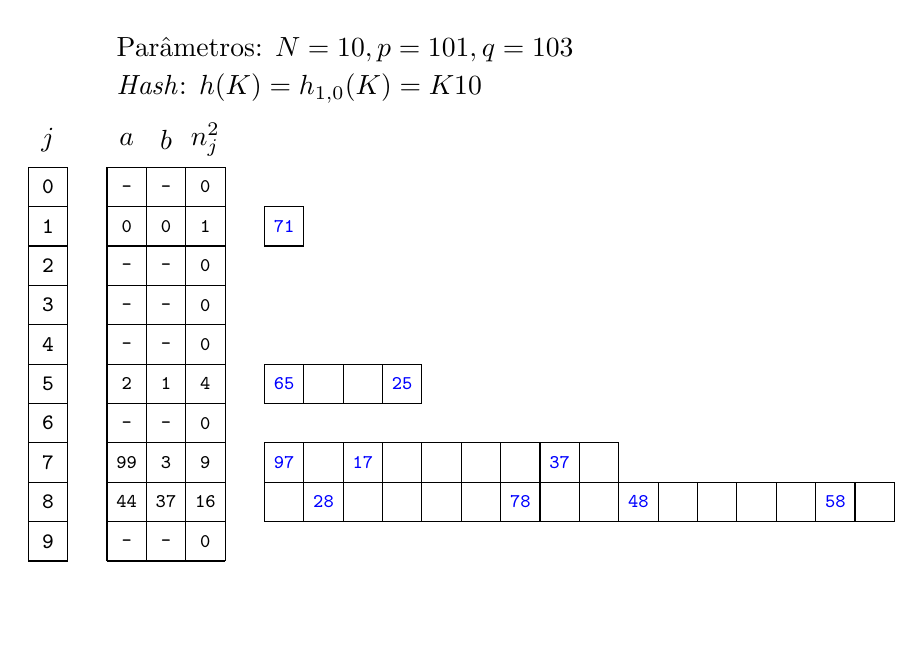
\begin{tikzpicture}
            \node[anchor=west] at (1, 6.5) { Parâmetros: $N = 10, p = 101, q = 103$ };
            \node[anchor=west] at (1, 6) { \textit{Hash}: $h(K) = h_{1,0}(K) = \Mod{K}{10}$ };

            \begin{scope}[scale=0.5]
                \node at (0.5, 10.7) { $j$ };
                \node at (2.5, 10.7) { $a$ };
                \node at (3.5, 10.7) { $b$ };
                \node at (4.5, 10.7) { $n_j^2$ };

                \node at (0.5, 9.5) { \footnotesize \tt \textbf{0} };
                \node at (0.5, 8.5) { \footnotesize \tt \textbf{1} };
                \node at (0.5, 7.5) { \footnotesize \tt \textbf{2} };
                \node at (0.5, 6.5) { \footnotesize \tt \textbf{3} };
                \node at (0.5, 5.5) { \footnotesize \tt \textbf{4} };
                \node at (0.5, 4.5) { \footnotesize \tt \textbf{5} };
                \node at (0.5, 3.5) { \footnotesize \tt \textbf{6} };
                \node at (0.5, 2.5) { \footnotesize \tt \textbf{7} };
                \node at (0.5, 1.5) { \footnotesize \tt \textbf{8} };
                \node at (0.5, 0.5) { \footnotesize \tt \textbf{9} };

                \node at (2.5, 9.5) { \scriptsize \tt - };
                \node at (3.5, 9.5) { \scriptsize \tt - };
                \node at (4.5, 9.5) { \scriptsize \tt 0 };

                \node at (2.5, 8.5) { \scriptsize \tt 0 };
                \node at (3.5, 8.5) { \scriptsize \tt 0 };
                \node at (4.5, 8.5) { \scriptsize \tt 1 };
                \node at (6.5, 8.5) { \scriptsize \tt \textcolor{blue}{71} };

                \node at (2.5, 7.5) { \scriptsize \tt - };
                \node at (3.5, 7.5) { \scriptsize \tt - };
                \node at (4.5, 7.5) { \scriptsize \tt 0 };

                \node at (2.5, 6.5) { \scriptsize \tt - };
                \node at (3.5, 6.5) { \scriptsize \tt - };
                \node at (4.5, 6.5) { \scriptsize \tt 0 };

                \node at (2.5, 5.5) { \scriptsize \tt - };
                \node at (3.5, 5.5) { \scriptsize \tt - };
                \node at (4.5, 5.5) { \scriptsize \tt 0 };

                \node at (2.5, 4.5) { \scriptsize \tt 2 };
                \node at (3.5, 4.5) { \scriptsize \tt 1 };
                \node at (4.5, 4.5) { \scriptsize \tt 4 };
                \node at (6.5, 4.5) { \scriptsize \tt \textcolor{blue}{65} };
                \node at (9.5, 4.5) { \scriptsize \tt \textcolor{blue}{25} };

                \node at (2.5, 3.5) { \scriptsize \tt - };
                \node at (3.5, 3.5) { \scriptsize \tt - };
                \node at (4.5, 3.5) { \scriptsize \tt 0 };

                \node at (2.5, 2.5) { \scriptsize \tt 99 };
                \node at (3.5, 2.5) { \scriptsize \tt 3 };
                \node at (4.5, 2.5) { \scriptsize \tt 9 };
                \node at (8.5, 2.5) { \scriptsize \tt \textcolor{blue}{17} };
                \node at (13.5, 2.5) { \scriptsize \tt \textcolor{blue}{37} };
                \node at (6.5, 2.5) { \scriptsize \tt \textcolor{blue}{97} };

                \node at (2.5, 1.5) { \scriptsize \tt 44 };
                \node at (3.5, 1.5) { \scriptsize \tt 37 };
                \node at (4.5, 1.5) { \scriptsize \tt 16 };
                \node at (7.5, 1.5) { \scriptsize \tt \textcolor{blue}{28} };
                \node at (15.5, 1.5) { \scriptsize \tt \textcolor{blue}{48} };
                \node at (20.5, 1.5) { \scriptsize \tt \textcolor{blue}{58} };
                \node at (12.5, 1.5) { \scriptsize \tt \textcolor{blue}{78} };

                \node at (2.5, 0.5) { \scriptsize \tt - };
                \node at (3.5, 0.5) { \scriptsize \tt - };
                \node at (4.5, 0.5) { \scriptsize \tt 0 };

                \draw (0,0) grid (1, 10);
                \draw (2,0) grid (5, 10);
                \draw (6,8) grid (7, 9);
                \draw (6,4) grid (10, 5);
                \draw (6,2) grid (15, 3);
                \draw (6,1) grid (22, 2);

                \draw[white] (0, -2);
            \end{scope}

        \end{tikzpicture}
    \end{figure}

\end{frame}


